\chapter{Evaluating Regression}
\label{ch:reg-eval}

The last lessons quickly introduced scoring for regression and essential measures such as RMSE and MAE. In classification, the confusion matrix was an excellent addition to finding misclassified data instances. But the confusion matrix could only be applied to discrete classes. Before Orange gets some similar for regression, one way to find misclassified data instances is through scatter plot!


\marginnote{\textbf{\textsf{This workflow visualizes the predictions that we have constructed on the training data. How would you change the widget to use a separate test set? Hint: The Sample widget can help.}}}

\begin{figure}[h]
    \centering
    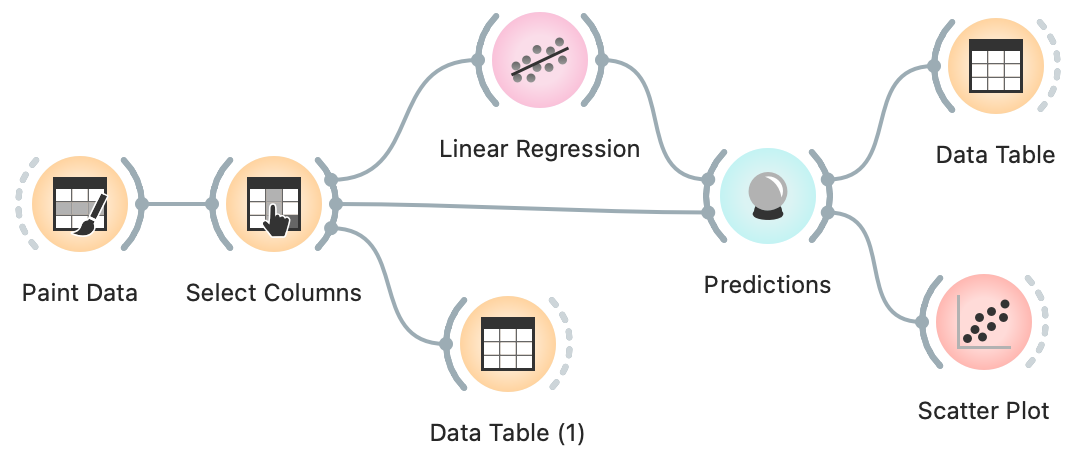
\includegraphics[scale=0.5]{workflow-predictions.png}
    \caption{$\;$}
\end{figure}

We can play around with this workflow by painting the data such that the regression would perform well on the blue data point and fail on the red outliers. In the scatter plot, we can check if the predicted and true class difference was what we had expected.

\begin{figure}[h]
    \centering
    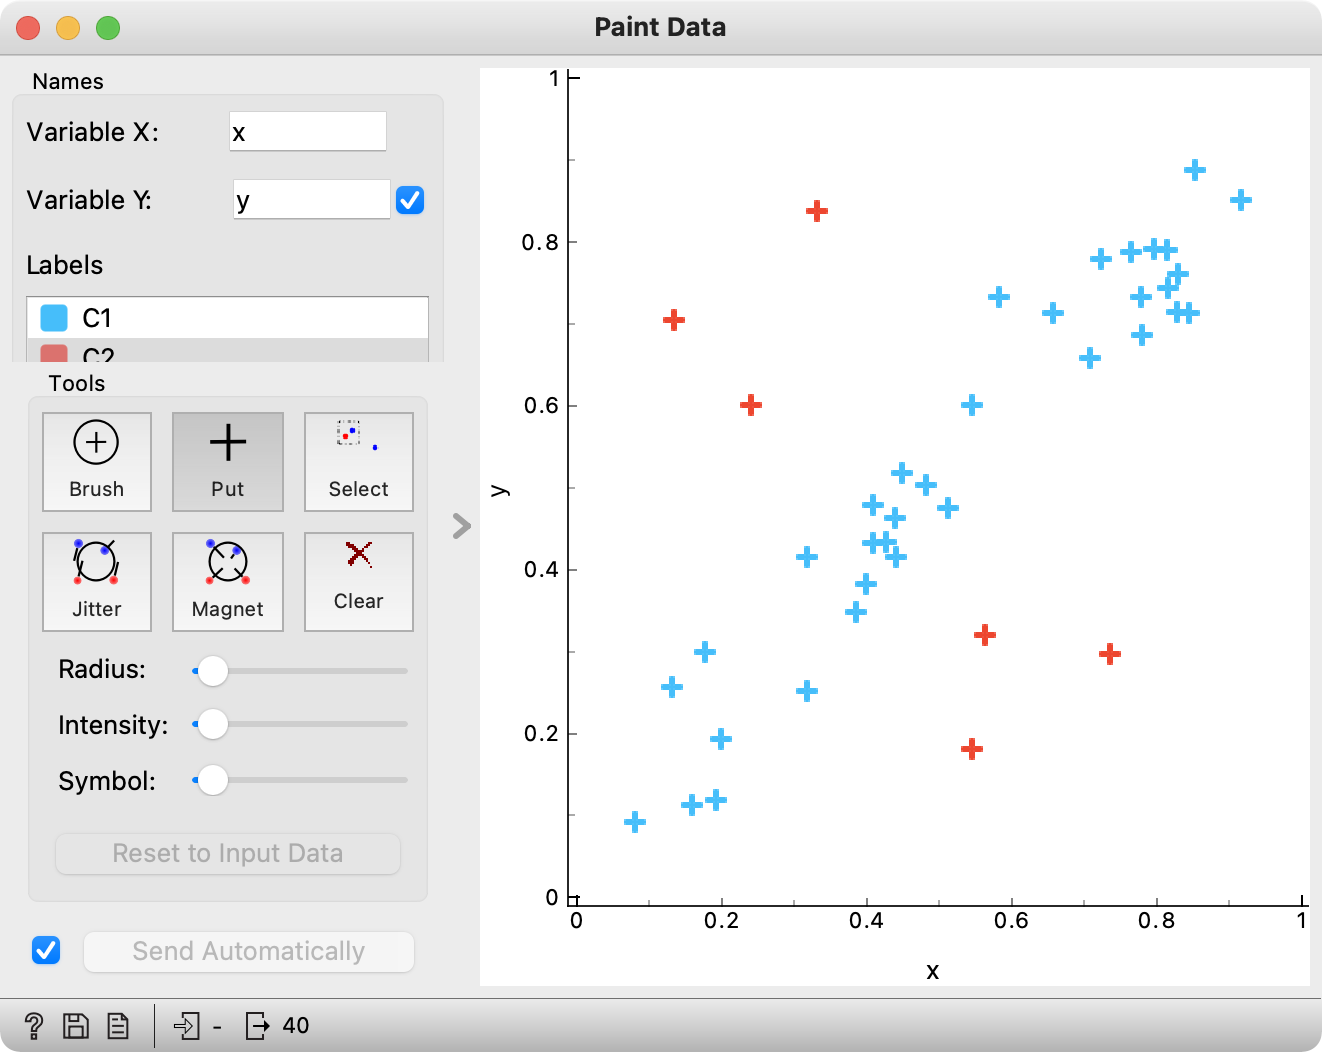
\includegraphics[scale=0.5]{paint.png}
    \caption{$\;$}
\end{figure}

A similar workflow would work for any data set—for instance, the housing data set (from Orange distribution). Say, just like above, we would like to plot the relationship between true and predicted continuous class, but would like to add information on the absolute error the predictor makes. Where is the error coming from? We need a new column. The Feature Constructor widget (albeit a bit geekish) comes to the rescue.

\begin{figure}[h]
    \centering
    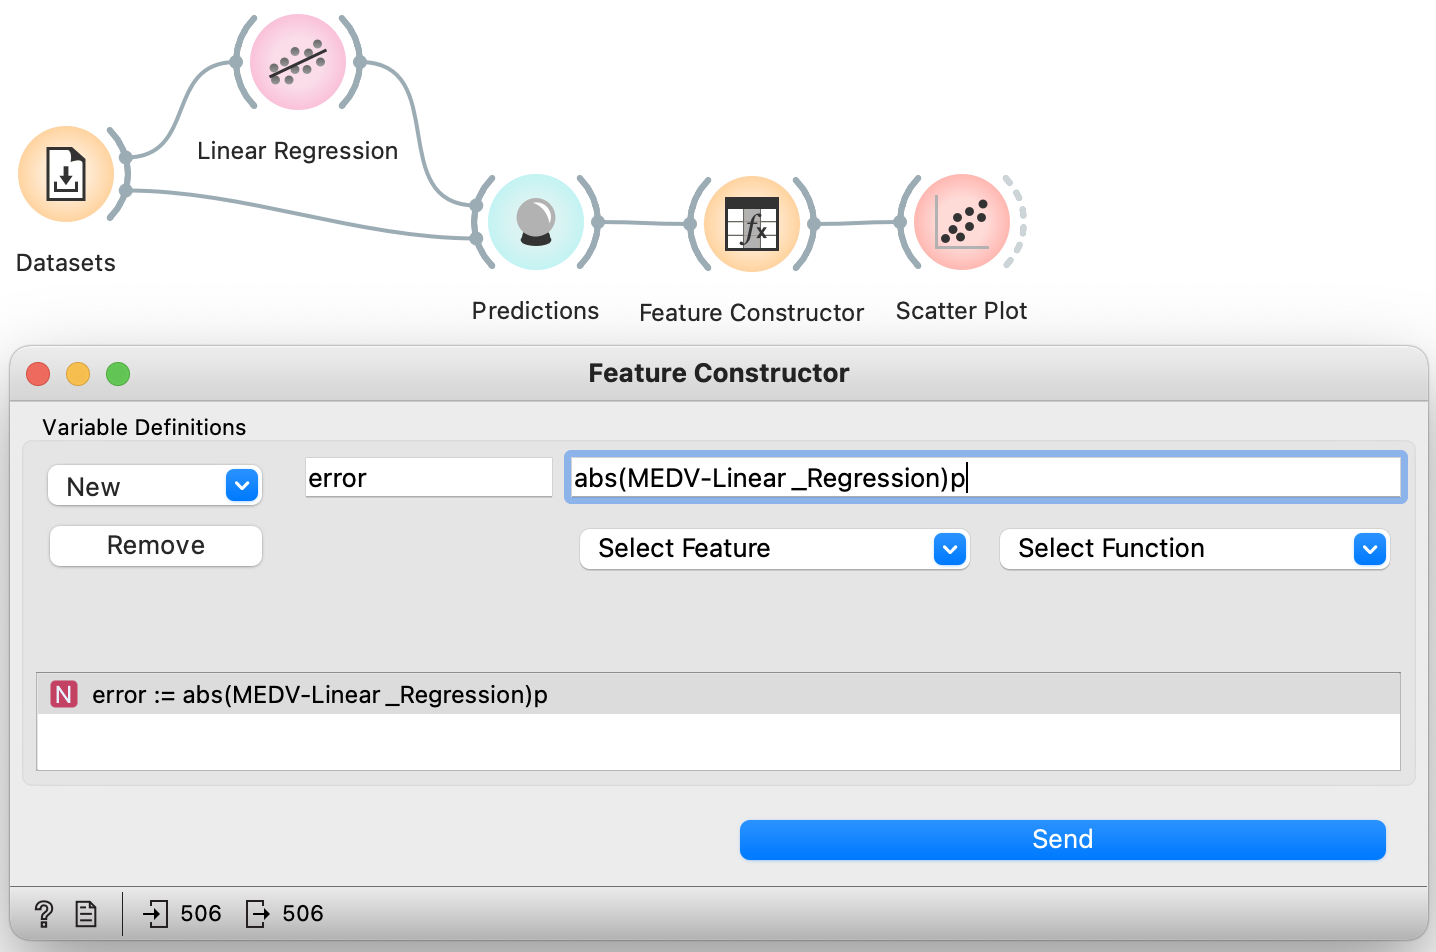
\includegraphics[scale=0.4]{feature-constructor.png}
    \caption{$\;$}
\end{figure}

In the \widget{Scatter Plot}, we can now select the data where the predictor erred substantially and explore the results further. 

\marginnote{\textbf{\textsf{We could, in principle, also mine the errors to see if we can identify data instances for which this was high. But then, if this is so, we could have improved predictions at such regions. Like, construct predictors that predict the error. Creating such predictors looks weird. Could we then also build a predictor that predicts the error of the predictor that predicts the error? Strangely enough, such ideas have recently led to something called Gradient Boosted Trees, which are nowadays among the best regressors. Check them out using the Gradient Boosting widget.}}}

\begin{figure}[h]
    \centering
    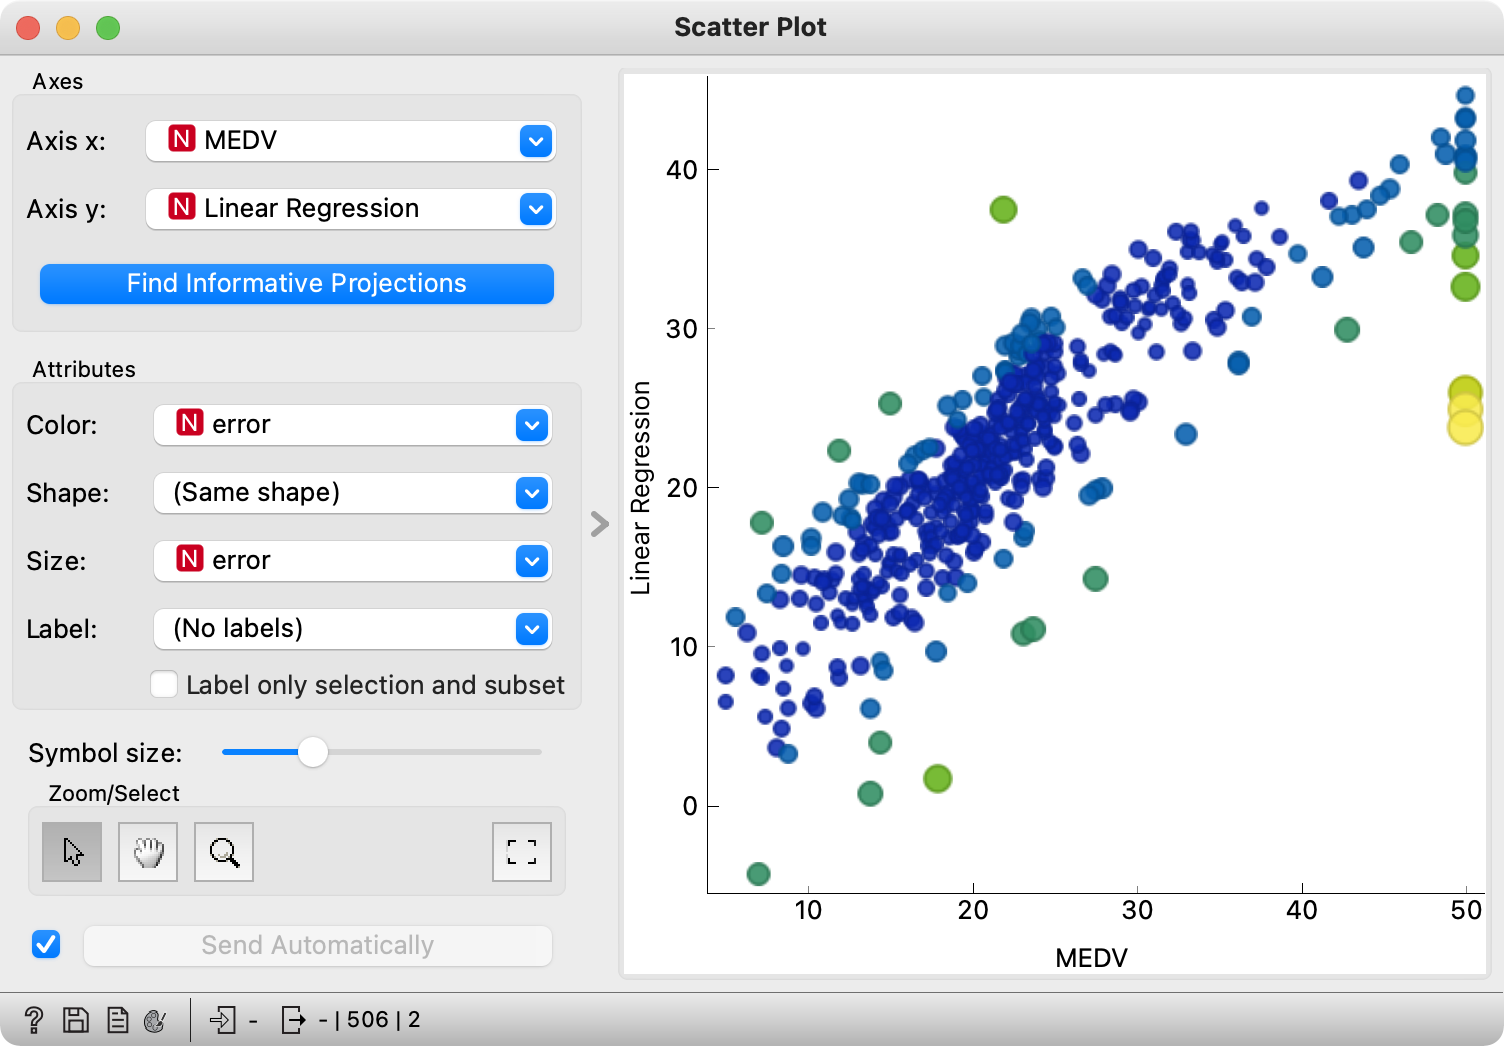
\includegraphics[scale=0.4]{scatterplot.png}
    \caption{$\;$}
\end{figure}